\documentclass[11pt,twocolumn]{article}
\usepackage[T1]{fontenc}
\usepackage[utf8]{inputenc}
\usepackage{mathptmx}
\renewcommand{\ttdefault}{lmtt}
\usepackage{amsmath,amssymb}
\usepackage[letterpaper,margin=0.9in,columnsep=0.3in,headheight=14pt]{geometry}
\usepackage{graphicx}
\usepackage{float}
\usepackage[labelfont=bf,textfont=bf,font=small,labelsep=colon]{caption}
\usepackage{titlesec}
\usepackage{enumitem}
\usepackage{fancyhdr}
\usepackage[hidelinks]{hyperref}

\graphicspath{{figures/}}
\setlength{\parindent}{1.5em}
\setlist{leftmargin=1.4em,itemsep=2pt,topsep=3pt}

\pagestyle{fancy}
\fancyhf{}
\fancyhead[R]{\thepage}
\renewcommand{\headrulewidth}{0pt}

\titleformat{\section}{\centering\LARGE\bfseries}{}{0pt}{}
\titleformat{\subsection}{\large\bfseries}{}{0pt}{}
\titlespacing*{\section}{0pt}{14pt}{8pt}
\titlespacing*{\subsection}{0pt}{10pt}{4pt}

\newcommand{\fn}[1]{\textit{#1}}
\newcommand{\level}[2]{\section*{\underline{LEVEL #1:} #2}}
\newcommand{\sub}[1]{\subsection*{#1}}
\newcommand{\figcap}[2]{\caption*{Figure #1: #2}}

\raggedbottom
\begin{document}

\twocolumn[
\begin{center}
{\fontsize{24}{28}\selectfont Multimedia Systems, Assignment 2025--2026\par}
\vspace{4pt}
Georgios Ioannidis, AEM: 10833\\
Panagiotis Charalampos Papadopoulos, AEM: 10898
\end{center}
\vspace{14pt}
]
\thispagestyle{fancy}

\level{1}{Sequence Segmentation Control \& Filterbank}

The implementation of the first level focuses on the analysis/synthesis architecture for achieving Perfect Reconstruction with the use of KBD windows.

\sub{1.1 Helper Functions}
To keep the code clean and reusable, the implementation relies on a set of helper functions:
\begin{itemize}
  \item \textbf{\fn{get\_kbd\_window(N, alpha), derive\_window(win\_type, N)}}: The Kaiser-Bessel Derived (KBD) windows are built by calling the \fn{kaiser} function of the \fn{scipy} library and computing the square root of the ratio of the partial sum to the total sum of the coefficients. The function \fn{derive\_window} acts as a control function, returning the appropriate window (with $\alpha=6.0$ for Long windows of $N=2048$ and $\alpha=4.0$ for Short windows of $N=256$).
  \item \textbf{\fn{mdct4(x), imdct4(x)}}: They form the core of the transform to the frequency domain and back. To implement the MDCT, \fn{mdct4} first applies the necessary folding of the signal through the operation \texttt{[-c[::-1]-d, a-b[::-1]]} and then calls the standard DCT. Correspondingly, \fn{imdct4} takes the result of the inverse transform and unfolds it to recover $2N$ samples, incorporating the necessary time-domain folding.
\end{itemize}

\sub{1.2 Frame Type Control (SSC Function)}
The SSC function decides the window type for each frame by detecting abrupt changes. The procedure consists of the following stages:
\begin{itemize}
  \item \textbf{\textit{Filtering \& Energy}}: The signal of the next frame passes through a high-pass filter. The result is divided into 8 segments of 128 samples and the energy of each segment is computed. If the energy of a segment exceeds the threshold $10^{-3}$ and is at the same time ten times the mean of the previous ones, an attack is detected in that channel and the flag for the transition to EIGHT\_SHORT\_SEQUENCE is set.
  \item \textbf{\fn{get\_channel\_type}}: The selection of the next state (so that transitions from Long to Short windows are smooth) was implemented through the inner helper function \fn{get\_channel\_type(prev\_type, next\_is\_esh)}. This function enforces the transition rules (e.g.\ OLS moves to LSS if a transient follows, and LSS always goes to ESH). The function is called independently for the left and the right channel. Finally, through the dictionary \fn{table\_1}, the two independent decisions are merged into the final, common window type of the current frame.
\end{itemize}

\sub{1.3 Window Handling (filter\_bank \& i\_filter\_bank)}
The function \fn{filter\_bank} organizes the transition to the frequency domain by applying the appropriate window shapes. It first calls \fn{derive\_window} to obtain the symmetric Long and Short windows. For each channel, depending on the frame type:
\begin{itemize}
  \item \textbf{OLS}: The symmetric window of 2048 samples is applied and the result is passed directly to the helper function \fn{mdct4}.
  \item \textbf{LSS / LPS}: The asymmetric windows are built dynamically and their product with the signal is again passed to \fn{mdct4}.
  \item \textbf{ESH}: The central part of the signal is split into 8 overlapping subframes (of 256 samples). For each subframe the short window is applied, and \fn{mdct4} is called 8 times in a row. The individual spectra are stacked vertically with \fn{np.concatenate}.
\end{itemize}
The inverse procedure is carried out symmetrically in \fn{i\_filter\_bank}, which calls \fn{imdct4} and applies overlap-add on the temporary buffer specifically for the ESH case.

\sub{1.4 Main Coding Loop (aac\_coder\_1 / i\_aac\_coder\_1)}
The main body coordinates the above procedure through the following steps:
\begin{itemize}
  \item \textbf{Padding Alignment}: Before processing, the code checks the length of the file. If it is not an integer multiple of 1024, zeros are appended at the end, so that no information from the last frame is lost.
  \item \textbf{Data Formatting}: The spectral data returned by \fn{filter\_bank} are organized in a list of dictionaries. Particular care is given to ESH frames, where the initially one-dimensional vector is strictly reshaped into a matrix of size (128, 8).
  \item \textbf{No Quantization}: The absence of quantization (which is introduced in the next levels) explains the Perfect Reconstruction property, which is confirmed by the SNR measurement.
\end{itemize}

\sub{1.5 Demonstration and Results (demo\_aac\_1)}
This is where the overall test of the coder takes place. The function runs a full compression and decompression cycle on the file, so that we can evaluate the final result both numerically (SNR computation) and visually (plots).

\sub{1.6 Discussion of Results}
The correct operation of the coder was evaluated with the audio file \fn{LicorDeCalandraca.wav} (48\,kHz, stereo). The results confirm that Perfect Reconstruction is achieved and that the individual algorithms behave correctly. The code was implemented in a Google Colab notebook.

First, the quantitative evaluation of the system was based on the computation of the Signal-to-Noise Ratio (SNR). In Level 1, the SNR was measured at 303.22\,dB for the left channel and 303.37\,dB for the right, with the total SNR at 303.30\,dB. This excellent result is also clearly reflected in the power measurements, where the error power (Noise Power) was recorded at negligible levels of the order of $10^{-32}$ ($1.64\times10^{-32}$ for the left and $1.69\times10^{-32}$ for the right channel), against the power of the useful signal ($3.45\times10^{-2}$ and $3.68\times10^{-2}$ respectively). Such SNR values are considered practically infinite in the context of digital signal processing and indicate that the output signal is mathematically identical to the input signal. The negligible error that remains is not due to algorithmic flaws. It comes only from the unavoidable rounding error introduced by double-precision floating-point operations.

\begin{figure}[H]
  \centering
  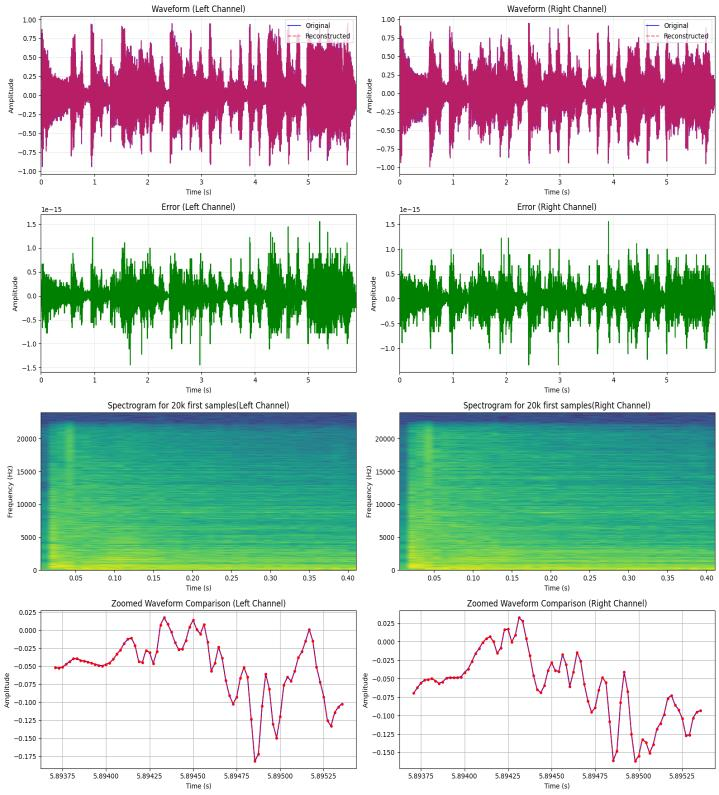
\includegraphics[width=\columnwidth]{fig_1_1_signal_analysis.png}
  \figcap{1.1}{Signal Analysis}
\end{figure}

The visual results of \textbf{Figure 1.1}, which shows the plots separately for the Left and the Right channel, confirm the above conclusions. The reconstructed waveform (red dashed line) fully overlaps the original one (blue line) in both channels, showing exact agreement in the time domain. The error signal plot shows that the deviations are of the order of $10^{-15}$, confirming the absence of error. In addition, the spectrogram gives a detailed picture of the energy distribution in the time-frequency domain for the first 20,000 samples. The colour map indicates the magnitude of the spectral coefficients. The bright shades (yellow and light green) correspond to regions with a high concentration of energy, which is normally found at the low frequencies of the audio signal, while the dark blue shades indicate the absence of significant acoustic energy. Vertical bright stripes can also be clearly seen, and these are the visual trace of the abrupt changes of the signal (transients). It is exactly these changes that the algorithm detects in order to activate the short windows (EIGHT\_SHORT\_SEQUENCE). Finally, the zoom on the last 80 samples shows that the zero padding during encoding and its removal (trimming) during decoding worked correctly and symmetrically, with no loss of information at the edges.

\begin{figure}[H]
  \centering
  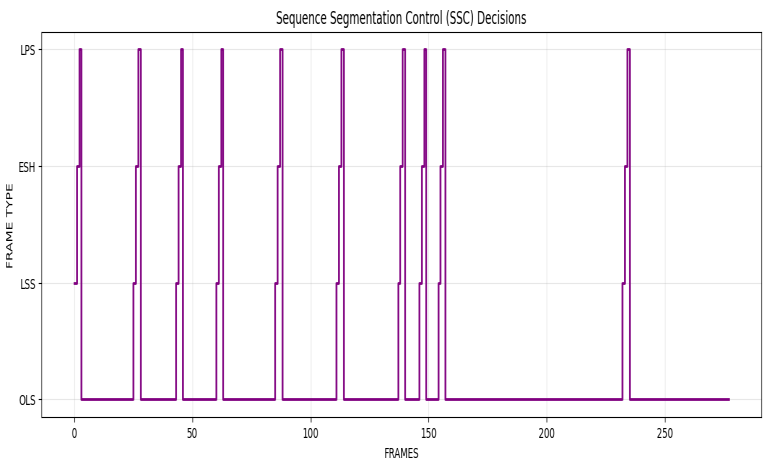
\includegraphics[width=\columnwidth]{fig_1_2_ssc_decisions.png}
  \figcap{1.2}{SSC Decisions}
\end{figure}

Regarding the dynamic behaviour of the coder, \textbf{Figure 1.2} shows the common final window type decided by the state machine of the Sequence Segmentation Control algorithm. During intervals where the signal is stationary, the coder steadily stays in the OLS state, using long windows for the best spectral resolution. In contrast, when abrupt energy changes are detected in either of the two channels, the algorithm moves to the short ESH windows through the intermediate LSS window and returns through LPS. This behaviour confines the quantization error in time to the region of the pulse, preventing the audible pre-echo effect.

\begin{figure}[H]
  \centering
  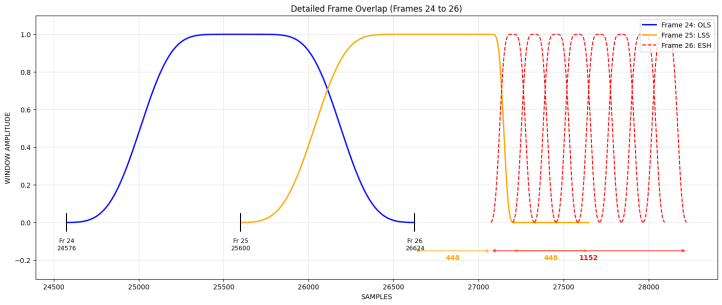
\includegraphics[width=\columnwidth]{fig_1_3_window_overlap.png}
  \figcap{1.3}{Detailed Window Overlap}
\end{figure}

Finally, the correct application of the windows is confirmed in Figure 1.3, which focuses on a typical transition region from OLS to LSS and then to ESH (Frames 24--26). The plot highlights the shape of the LSS window, which starts smoothly to match the preceding OLS, keeps a flat region of 448 samples equal to one, and then ends abruptly. This leaves exactly the space needed for the 8 short overlapping windows of the ESH type.

\level{2}{Temporal Noise Shaping (TNS)}

The implementation of the second level introduces the TNS (Temporal Noise Shaping) stage, which aims to control the temporal distribution of the quantization noise. At this stage the MDCT coefficients are processed but not quantized, so the system remains practically lossless.

\sub{2.1 Table \& Band Handling}
The TNS parameters are based on the tables of the standard, which are loaded from the file \fn{TableB219.mat}. The function \fn{load\_tns\_tables} separates the tables into:
\begin{itemize}
  \item \textbf{B219a} (for long windows of 2048 samples -- OLS/LSS/LPS)
  \item \textbf{B219b} (for windows of 256 samples -- ESH).
\end{itemize}
The TNS band limits (starts, ends) are then extracted dynamically from these tables, so that filtering is applied to the appropriate spectral regions. For ESH frames, the MDCT coefficients are rearranged using:\\
\texttt{reshape(128, 8, order='F').T}\\
so that the 8 subframes are processed independently.

\sub{2.2 TNS Analysis -- Encoder (tns Function)}
The Temporal Noise Shaping procedure is implemented through two complementary functions that handle encoding (analysis) and decoding (synthesis) independently for each channel and subframe:

\textbf{A. Analysis Procedure (Encoder -- \fn{tns}):}
\begin{enumerate}
  \item \textbf{Normalization}: The energy $P_b$ of each TNS band is computed. The weight array $S_w=\sqrt{P_b}$ is created and smoothed with a moving average to avoid abrupt changes. The spectrum is normalized as $X_w = X_k / S_w$.
  \item \textbf{LPC Coefficient Computation}: Autocorrelation is applied to the normalized spectrum (\fn{np.correlate}). The linear prediction coefficients are obtained by solving the system $R\mathbf{a}=\mathbf{r}$, using the function \fn{scipy.linalg.solve} and a Toeplitz matrix.
  \item \textbf{Quantization and Check}: The coefficients are quantized with a step of 0.1 and limited to the interval $[-0.8, 0.7]$ (\fn{np.clip}). A stability check is performed through the roots of the polynomial (\fn{numpy.polynomial.Polynomial}). If a root with magnitude greater than 1.0 is found, the filter is considered unstable and the coefficients are set to zero.
  \item \textbf{FIR Filtering}: The original spectrum is filtered with the function \fn{lfilter} (used as an FIR filter), producing the residual signal.
\end{enumerate}

\textbf{B. Synthesis Procedure (Decoder -- \fn{i\_tns}):}
\begin{itemize}
  \item \textbf{Inverse Filtering (IIR)}: To restore the original spectrum, the function takes the modified signal (residual) and applies exactly the inverse procedure. This is done by using \fn{lfilter} again, feeding it the same quantized coefficients that the encoder computed and sent.
  \item \textbf{Restoring Dimensions}: Once filtering is complete, the dimensions are restored (flattening with the parameter \texttt{order='F'}) for the exact reconstruction of the original form of the MDCT matrix. This allows a smooth transition to the inverse filterbank stage.
\end{itemize}

\sub{2.3 Main Encoding \& Decoding Loop (aac\_coder\_2 / i\_aac\_coder\_2)}
Integrating TNS into the main processing loop changes the data flow of the system. In encoding (\fn{aac\_coder\_2}), after the window type is determined (through the SSC stage) and the signal is moved to the frequency domain (through \fn{filter\_bank}), the MDCT coefficients are passed to the \fn{tns} function. The procedure is carried out independently for the left and the right channel. The output dictionary of each frame now also contains the quantized linear prediction coefficients (\fn{tns\_coeffs}), while the \fn{frame\_F} field now stores the filtered coefficients (the residual signal) instead of the original spectrum.

Conversely, during decoding (\fn{i\_aac\_coder\_2}), the system retrieves the TNS coefficients and the residual signal from the data structure. The function \fn{i\_tns} is called for each channel and applies the inverse IIR filter, so that the original MDCT spectrum is reconstructed. The data are then reshaped appropriately (with \fn{flatten}) and fed to the \fn{i\_filter\_bank} stage for the transition to the time domain and the final synthesis through overlap-add.

\sub{2.4 Demonstration and Evaluation (demo\_aac\_2)}
The function \fn{demo\_aac\_2} coordinates the complete execution of the second level and handles both the quantitative measurement and the visualization of the TNS performance. First, it aligns the original and the decoded file in time (removing the padding) and computes the error signal. Based on this, it computes the Signal-to-Noise Ratio (SNR) for each channel separately and overall, confirming the mathematical invertibility of the procedure. In addition, the function searches within the \fn{aac\_seq\_2} structure for frames where TNS was highly active and dynamically reconstructs the original spectrum, in order to produce the comparative diagnostic plots (spectrum, prediction gain and reconstruction error).

\sub{2.5 Discussion of Results}
The operation of TNS was evaluated by encoding and decoding the two-channel input file. The quantitative evaluation showed that the system keeps the Perfect Reconstruction property. Specifically, the SNR was measured at 303.20\,dB for the left channel and 303.35\,dB for the right, with the total SNR at 303.28\,dB. These practically infinite values confirm that the TNS analysis (FIR) and synthesis (IIR) are fully inverted, since the negligible error observed is limited to machine precision and no audible distortion is introduced.

The plots produced by the run are discussed below:

\begin{figure}[H]
  \centering
  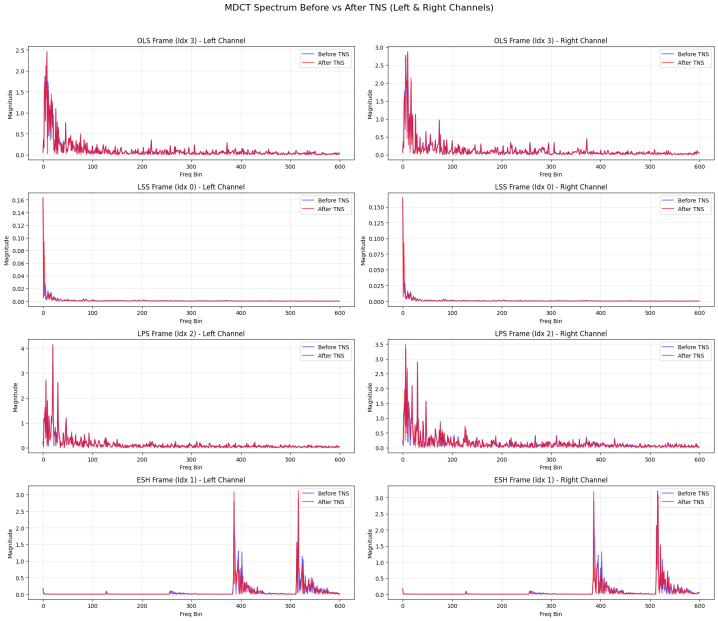
\includegraphics[width=\columnwidth]{fig_2_1_mdct_spectrum_tns.png}
  \figcap{2.1}{MDCT Spectral Analysis (Before and After TNS)}
\end{figure}

\begin{itemize}[label=$\blacktriangleright$]
  \item In the OLS (Index 3) and LPS (Index 2) frames, the TNS filter slightly modifies the spectral envelope in both channels, mainly at the low frequencies where the energy is concentrated.
  \item In the ESH frame (Index 1), which is characterized by strong changes in the time domain, the effect of TNS is strong. The filtered signal (red line) shows clear differences at the peaks compared to the original one (blue line). This shows that the prediction filter successfully ``whitened'' the spectrum. It removed the predictable structure and moved information from the frequency domain to the time domain, in order to counter quantization noise spreading.
  \item In the LSS frame (Index 0), the effect is smaller, since the signal in that time window appears to have lower energy and a less pronounced spectral structure.
\end{itemize}

\begin{figure}[H]
  \centering
  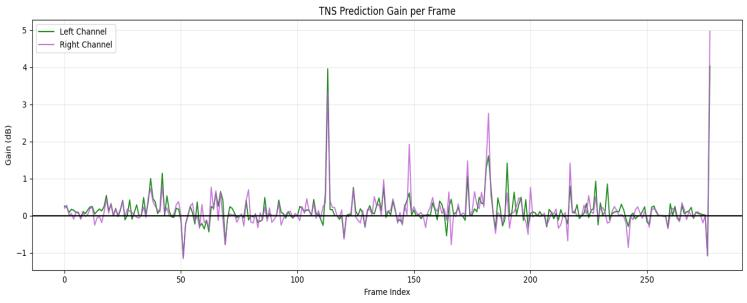
\includegraphics[width=\columnwidth]{fig_2_2_tns_prediction_gain.png}
  \figcap{2.2}{TNS Prediction Gain}
\end{figure}

The plot of Figure 2.2 shows the prediction gain per frame for the Left (green line) and the Right channel (purple line) at the same time. Positive values indicate that the TNS filter managed to predict the signal correctly, removing redundant information and reducing the energy of the coefficients to be encoded.
\begin{itemize}[label=$\blacktriangleright$]
  \item Strong simultaneous spikes appear in both channels, often exceeding 4\,dB (e.g.\ near frame 115 and frame 275). These peaks correspond in time to the points of the signal with the strongest transients, where the contribution of TNS is at its maximum.
  \item In the parts where the signal is stationary, the gain stays close to zero, since linear prediction in the frequency domain offers no significant advantage when there are no abrupt changes in time. In a few cases slightly negative values also appear. These are due to the limitations imposed by the quantization of the coefficients (to 4 bits).
\end{itemize}

\begin{figure}[H]
  \centering
  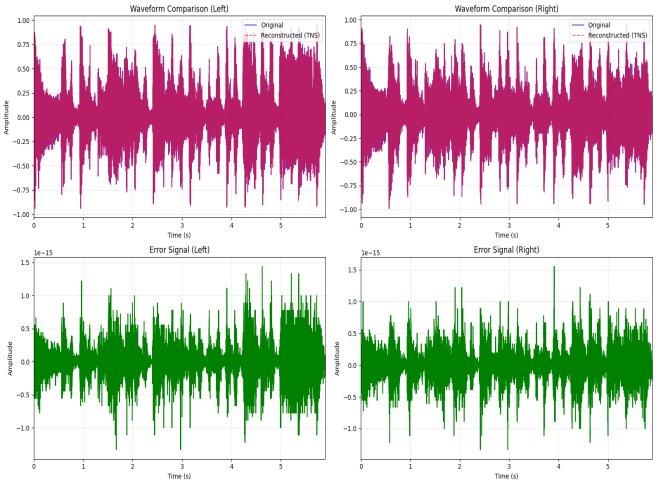
\includegraphics[width=\columnwidth]{fig_2_3_waveform_error.png}
  \figcap{2.3}{Waveform Comparison and Error Signal}
\end{figure}

\begin{itemize}[label=$\blacktriangleright$]
  \item In the upper plots (Waveform Comparison), the reconstructed waveform (red dashed line) matches the original one (solid blue) exactly in both channels, so the two are practically indistinguishable.
  \item In the lower plots (Error Signal), the reconstruction error ($x_{\text{original}} - x_{\text{reconstructed}}$) is of the order of $10^{-15}$. This error level is negligible and is due only to the finite precision of floating-point operations during the application of the successive filters (FIR in analysis and IIR in synthesis). The amplitude of the error confirms that the TNS procedure is fully inverted.
\end{itemize}

\level{3}{Psychoacoustic Model \& Quantization}

The implementation of the third level completes the coder and turns it into a full lossy system. The main principle relies on exploiting the imperfections of the human ear through a Psychoacoustic Model. The noise that is unavoidably introduced during quantization is now ``hidden'' below the masking threshold, which allows a drastic reduction of the bitrate without perceptible loss of quality. Finally, the data are compressed losslessly with entropy coding (Huffman).

\sub{3.1 Psychoacoustic Model (psycho)}
This stage takes the signal in the time domain and computes the Signal-to-Mask Ratio (SMR). It returns a $69\times1$ vector for the long windows (OLS, LSS, LPS) and a $42\times8$ matrix for ESH. To keep the architecture efficient, the procedure is supported by the following helper functions:
\begin{itemize}
  \item \textbf{\fn{precompute\_spreading\_function}}: Computes the masking spreading matrices only once, at the start of the program. This way the computationally heavy operations are not repeated for every frame, which improves the speed of the coder dramatically.
  \item \textbf{\fn{psycho\_one\_window}}: This is the computational core for each window ($N=2048$ or $N=256$). The computation starts with the \textbf{Spectral Analysis}, where the signal is multiplied by a Hann window and transformed with the FFT (\fn{scipy.fft.fft}) to obtain the magnitude $r(\omega)$ and the phase $\varphi(\omega)$. Next, the \textbf{Predictability} of the signal is estimated through linear prediction from the two previous frames ($r_{\text{pred}} = 2r_{t-1} - r_{t-2}$ and $\varphi_{\text{pred}} = 2\varphi_{t-1} - \varphi_{t-2}$), and the deviation of the current spectrum from this prediction defines the unpredictability measure $c(\omega)$. Finally, in the \textbf{Energy \& Threshold} part, the energy $e(b)$ and the weighted predictability of each band are combined with the spreading matrix to compute the final tonality $tb = -0.299 - 0.43\ln(c)$. This value determines whether the band behaves more like a tone or like noise, and it sets the required SNR dynamically between 6\,dB and 18\,dB.
\end{itemize}

\textbf{Dynamic Handling of ESH Frames:}

In the main function \fn{psycho}, particular attention was paid to the temporal consistency of the eight subframes of an ESH frame. Since the standard requires the data of the two previous time instants (with a step of 128 samples) to compute the prediction, a ``memory'' (buffer) mechanism was developed.
\begin{itemize}
  \item For the \textbf{first subframe} ($k=0$), the code retrieves the data from the end of the previous long frame.
  \item For the \textbf{following subframes} ($k=1\ldots7$), the prediction is based on the immediately preceding subframes of the \textit{current} frame.
\end{itemize}
This dynamic selection ensures that the tonality analysis follows the actual time evolution of the signal, preventing errors that would lead to a wrong SMR.

The final SMR is obtained as the ratio of the signal energy to the masking threshold $T(b)$. The Absolute Threshold of Hearing is included in the computation of $T(b)$, while the constant EPS is used to stabilize the logarithmic computations and to avoid division by zero in cases of complete silence.

\sub{3.2 Non-Uniform Quantizer (aac\_quantizer)}
The quantizer is the stage where the actual compression of the data takes place, as it converts the MDCT coefficients into integer quantization symbols. More specifically, it handles the bit allocation by optimizing the Scale Factor of each band, so that the noise does not exceed the psychoacoustic threshold. It is supported by the following helper functions:
\begin{itemize}[label=$\blacktriangleright$]
  \item \textbf{\fn{quantize\_coeffs / dequantize\_coeffs}}: They implement the non-linear Equations (12) and (13) of the standard (including the Magic Number 0.4054).
\end{itemize}
{\footnotesize
\begin{align}
S(k) &= \operatorname{sgn}(X(k))\,\operatorname{int}\!\left[\left(|X(k)|\times2^{-\frac{1}{4}\alpha}\right)^{\frac{3}{4}}+\text{MagicNumber}\right] \tag{12}\\
\hat{X}(k) &= \operatorname{sgn}(S(k))\,|S(k)|^{\frac{4}{3}}\times2^{\frac{1}{4}\alpha} \tag{13}
\end{align}
}

\textbf{Scale Factor Search Algorithm ($\alpha$):}\\
The best $\alpha$ for each scalefactor band is found with an iterative strategy:
\begin{enumerate}
  \item \textbf{Initial Estimate}: A starting value $\hat{\alpha}$ is computed from the maximum MDCT coefficient of the frame and the parameter $MQ=8191$, which defines the maximum allowed quantization levels.
  \item \textbf{Optimization Loop}: The value of $\alpha$ is increased step by step as long as the quantization error power $P_e(b)$ stays below the hearing threshold $T(b)$ set by the psychoacoustic model.
\end{enumerate}

\textbf{Zeroing Criterion:} An extra check was added so that, if all coefficients of the band are quantized to zero (\texttt{if np.all(s\_band == 0)}), the loop terminates immediately. This prevents the pointless increase of $\alpha$ in very low-energy bands that have already ``gone silent''. In this way the algorithm stays stable and overflow of the values is avoided.

\textbf{Scale Factor Difference Limit ($\leq 60$):} According to the standard, the difference of $\alpha$ between neighbouring bands must not exceed 60. When a correction is needed, we chose to always lower the larger value (and not raise the smaller one). The reason is simple: a smaller $\alpha$ also means lower quantization noise. In this way we are fully sure that the noise will stay below the hearing threshold and will never be heard.

\textbf{Data Output:} Finally, the function outputs the Global Gain ($G=\alpha(0)$) and the differential values of the scale factors (sfc) for DPCM coding. The quantization symbols $S$ are formatted into a $1024\times1$ matrix, ready to be processed by the Huffman stage.

\sub{3.3 Huffman Coding Integration}
Entropy coding is carried out by importing the external library provided with the assignment (\fn{huff\_utils}). The Scale Factors undergo DPCM and are encoded with Codebook 11. During decoding (\fn{i\_aac\_coder\_3}), a zero-padding mechanism was applied, so that cases where the Huffman algorithm omits zero symbols at the edges of the spectrum are handled without problems.

\sub{3.4 Main Encoding \& Decoding Loop (aac\_coder\_3 / i\_aac\_coder\_3)}
The move from the second to the third level changes the main loop of the system radically, since the signal is now converted from floating-point form into a bitstream. More specifically, the following operations were added to the new loop:
\begin{itemize}
  \item \textbf{Psychoacoustic Model Integration}: The signal, after passing through the Filterbank and TNS (as in Level 2), is fed to the \fn{psycho} function.
  \item \textbf{Quantization \& Huffman}: The spectrum after TNS and the computed SMR are fed to \fn{aac\_quantizer}. The resulting integer MDCT coefficients ($S$) and the Scale Factors (sfc) are then compressed by the \fn{encode\_huff} function.
\end{itemize}
During reconstruction (\fn{i\_aac\_coder\_3}), the path is reversed with the addition of the corresponding new stages. The algorithm retrieves the bitstreams from the dictionary, decodes the Huffman symbols and passes the integer data to the \fn{i\_aac\_quantizer} function for dequantization.

Once the floating-point spectrum (MDCT floats) has been recovered, the flow continues exactly as in Level 2, calling \fn{i\_tns} and \fn{i\_filter\_bank} in turn.

\sub{3.5 System Demonstration and Evaluation (demo\_aac\_3)}
Unlike the second level, where the goal was perfect (lossless) reconstruction, the function \fn{demo\_aac\_3} evaluates the system as a full lossy coder, aiming at the right balance between quality and compression rate.

First, as in Level 2, the function coordinates the complete flow (encoding and decoding), aligns the signals and computes the SNR. However, the most important new addition is the quantitative measurement of compression. The algorithm goes through the final \fn{aac\_seq\_3} structure and sums the lengths of all generated binary sequences (Huffman bitstreams for sfc and stream). From this sum and the duration of the track, two new metrics are derived: the final Bitrate (in kbps) and the Compression Ratio. Finally, the results are visualized through a dedicated plotting function.

\sub{3.6 Experimental Results \& Evaluation (Level 3)}
Running the complete compression and decompression procedure (\fn{demo\_aac\_3}) produced the following quantitative results:
\begin{itemize}
  \item \textbf{Final SNR}: 8.83\,dB (Left channel) / 8.52\,dB (Right channel) -- Total: 8.67\,dB.
  \item \textbf{Average Bitrate}: 214.57\,kbps.
  \item \textbf{Compression Ratio}: 7.16:1.
\end{itemize}

\textbf{Discussion of the Quantitative Data:}\\
Unlike the previous levels (where the SNR tended to infinity), the seemingly ``low'' value of 8.67\,dB confirms the operation of the Psychoacoustic Model. It shows that the algorithm introduced controlled quantization noise to save space, but at the same time shaped it in frequency so that it is hidden below the hearing threshold. At the same time, the original amount of data was drastically reduced by \textbf{86\%} (Compression Ratio \textbf{7.16:1}), with the final bitrate at 214.57\,kbps (from 1536\,kbps originally), without any perceptible audible distortion.

The success of the method is also shown by the visual analysis of the generated plots:

\begin{figure}[H]
  \centering
  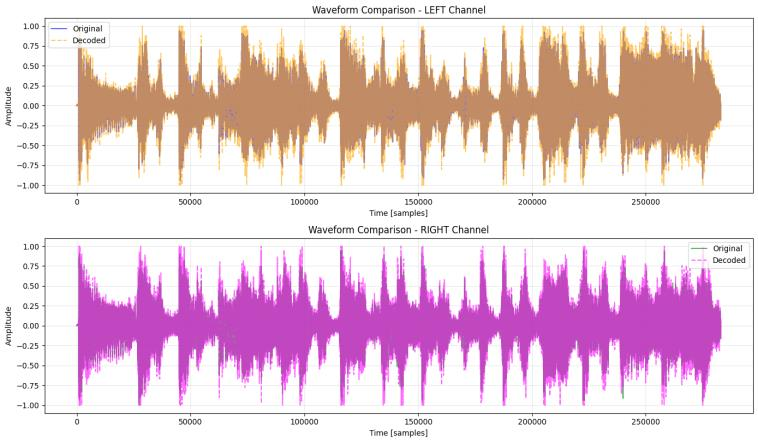
\includegraphics[width=\columnwidth]{fig_3_1_waveform_comparison.png}
  \figcap{3.1}{Waveform Comparison}
\end{figure}

\begin{figure}[H]
  \centering
  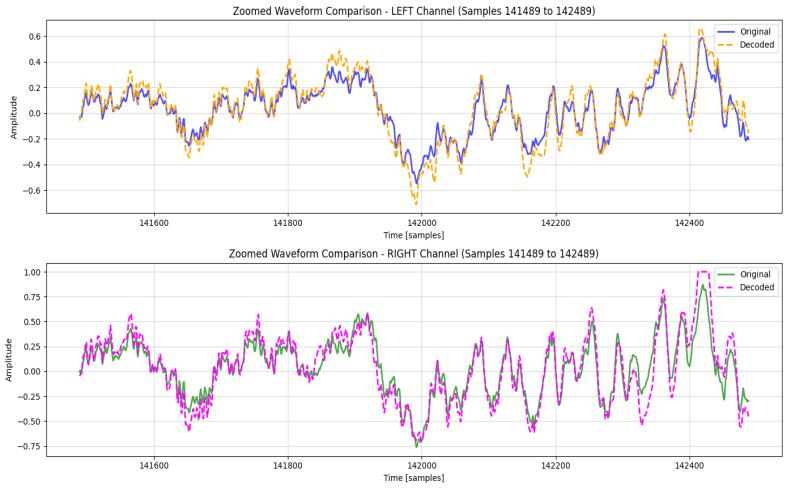
\includegraphics[width=\columnwidth]{fig_3_2_waveform_zoomed.png}
  \figcap{3.2}{Waveform Comparison (Zoomed)}
\end{figure}

\begin{figure}[H]
  \centering
  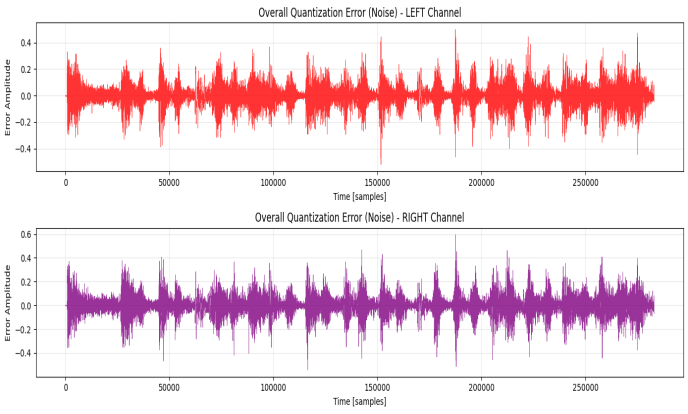
\includegraphics[width=\columnwidth]{fig_3_3_quantization_error.png}
  \figcap{3.3}{Overall Quantization Error}
\end{figure}

\begin{itemize}
  \item \textbf{Figure 3.1:} The reconstructed waveform matches the original one at the macroscopic level, confirming that the overall structure of the signal is preserved.
  \item \textbf{Figure 3.2:} In the zoomed view, a small but visible deviation can be seen in the amplitude of the reconstructed signal. This difference is the normal consequence of lossy compression and is due to the quantization process. Although the decoded line does not coincide exactly with the original one, it closely follows its trajectory, which shows that the coder preserves audio fidelity.
  \item \textbf{Figure 3.3:} The main difference shows up in the error signal, which is limited to values in the range $[-0.6, 0.6]$. This is essentially the deliberately shaped quantization noise (noise shaping), which is distributed in such a way that it never exceeds the audibility limit of human hearing in each frequency band.
\end{itemize}

\begin{figure}[H]
  \centering
  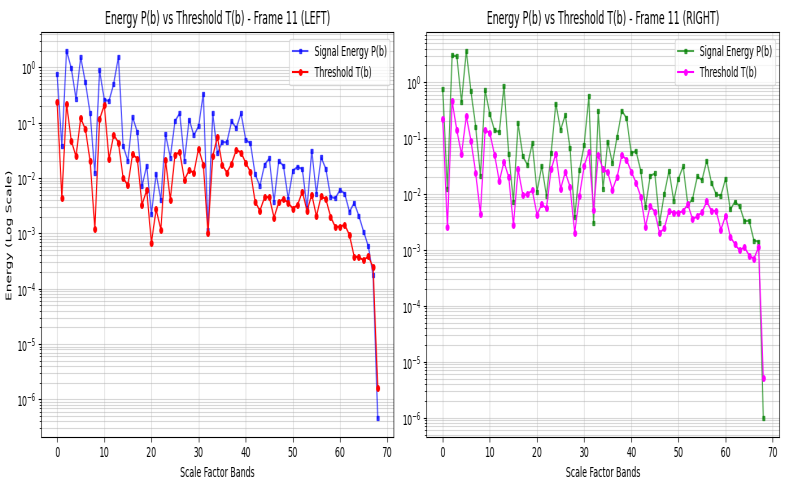
\includegraphics[width=\columnwidth]{fig_3_4_energy_vs_threshold.png}
  \figcap{3.4}{Energy P(b) vs Threshold T(b)}
\end{figure}

The plot of Figure 3.4, on a logarithmic scale, is a clear indication of the correct behaviour of the quantizer. The peaks of the signal energy (green/blue line) pull the masking threshold (purple/red line) upwards. It can be clearly seen that the quantizer is well tuned, as it keeps the noise just below the allowed limit in almost all frequency bands and thus optimizes compression.

\begin{figure}[H]
  \centering
  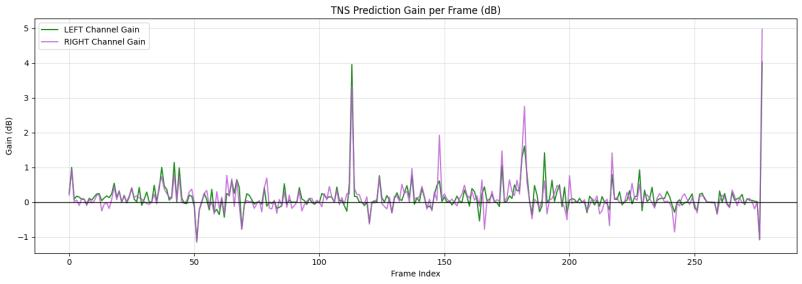
\includegraphics[width=\columnwidth]{fig_3_5_tns_gain_level3.png}
  \figcap{3.5}{TNS Prediction Gain per Frame (dB)}
\end{figure}

Figure 3.5 confirms that the Temporal Noise Shaping mechanism works smoothly together with the quantization system of Level 3. Significant gain peaks (spikes reaching 4--5\,dB) appear exactly at the points where the signal shows transients. At these time instants, TNS effectively ``whitens'' the spectrum. This reduces the correlation between the spectral coefficients and helps the quantizer distribute the available bits more efficiently.

\begin{figure}[H]
  \centering
  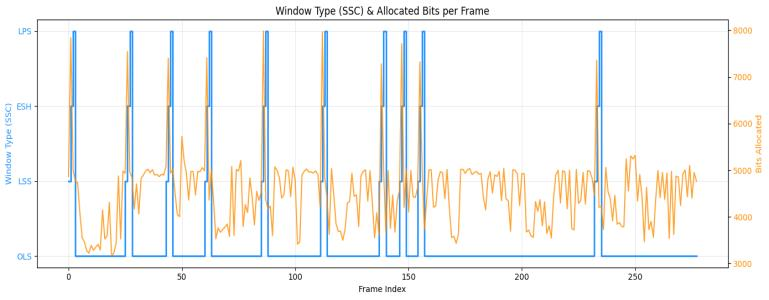
\includegraphics[width=\columnwidth]{fig_3_6_window_type_bits.png}
  \figcap{3.6}{Window Type (SSC) \& Allocated Bits per Frame}
\end{figure}

Figure 3.6 clearly shows the dynamic behaviour of both the window selection mechanism (SSC) and the entropy coding algorithm. A direct correlation can be observed. In the intervals where the SSC engine selects ESH windows (to protect against pre-echo), the required number of bits rises sharply (peaks above 7000--8000 bits), since 8 independent subframes have to be encoded. In contrast, in OLS frames the psychoacoustic model works more aggressively and brings the requirement down to 3500--4500 bits, which keeps the average bitrate of the system at the very good level of 214\,kbps.

\end{document}
